%% Standalone source for Figure 3 -- ATSR - GSQ estimates across analyses.
%% GENERATED by research/generate_revision_figures.py from the operative analysis
%% (analysis-results.json). Do not hand-edit; re-run the script.
%% Compile with tectonic/pdflatex -> fig3-atsr-gsq-forest.pdf.
\documentclass[border=4pt]{standalone}
\usepackage{pgfplots}
\pgfplotsset{compat=1.18}
\begin{document}
  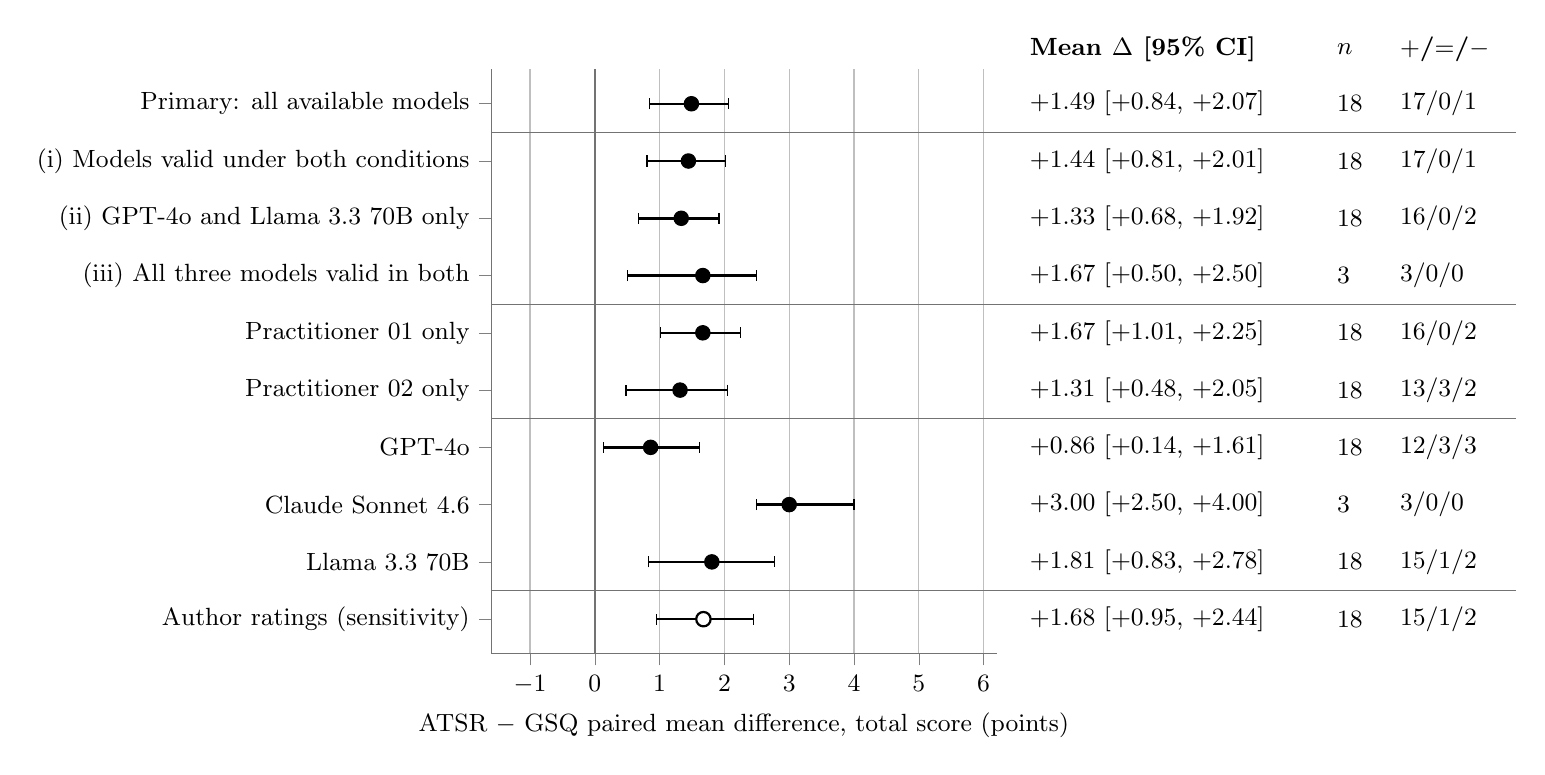
\begin{tikzpicture}
    \begin{axis}[
      width=8.0cm,
      height=9.0cm,
      xmin=-1.6, xmax=6.2,
      xtick={-1,0,1,2,3,4,5,6},
      xlabel={ATSR $-$ GSQ paired mean difference, total score (points)},
      xlabel style={font=\small},
      xticklabel style={font=\small},
      ymin=0.4, ymax=10.6,
      ytick={1,...,10},
      yticklabels={{Author ratings (sensitivity)},{Llama 3.3 70B},{Claude Sonnet 4.6},{GPT-4o},{Practitioner 02 only},{Practitioner 01 only},{(iii) All three models valid in both},{(ii) GPT-4o and Llama 3.3 70B only},{(i) Models valid under both conditions},{Primary: all available models}},
      yticklabel style={font=\small, align=right},
      xmajorgrids=true,
      grid style={black!25, line width=0.4pt},
      tick align=outside,
      axis line style={black!55},
      axis x line*=bottom,
      axis y line*=left,
      clip=false,
    ]
      %% zero reference (solid hairline, slightly darker than the grid)
      \draw[black!55, line width=0.6pt] (axis cs:0,0.4) -- (axis cs:0,10.6);
      \draw[black!55, line width=0.4pt] (axis cs:-1.6,9.5) -- ([xshift=66mm]axis cs:6.2,9.5);
      \draw[black!55, line width=0.4pt] (axis cs:-1.6,6.5) -- ([xshift=66mm]axis cs:6.2,6.5);
      \draw[black!55, line width=0.4pt] (axis cs:-1.6,4.5) -- ([xshift=66mm]axis cs:6.2,4.5);
      \draw[black!55, line width=0.4pt] (axis cs:-1.6,1.5) -- ([xshift=66mm]axis cs:6.2,1.5);
      \addplot[only marks, mark=none, error bars/.cd, x dir=both, x explicit,
               error bar style={black, line width=0.9pt}, error mark options={rotate=90, mark size=2pt, black}]
        coordinates { (1.490741,10) -= (0.652778,0) += (0.578704,0) (1.444444,9) -= (0.638889,0) += (0.569444,0) (1.333333,8) -= (0.652778,0) += (0.583333,0) (1.666667,7) -= (1.166667,0) += (0.833333,0) (1.666667,6) -= (0.657407,0) += (0.583333,0) (1.314815,5) -= (0.833333,0) += (0.731481,0) (0.861111,4) -= (0.722222,0) += (0.750000,0) (3.000000,3) -= (0.500000,0) += (1.000000,0) (1.805556,2) -= (0.972222,0) += (0.972222,0) (1.675926,1) -= (0.722222,0) += (0.768750,0) };
      \addplot[only marks, mark=*, mark size=2.6pt, mark options={fill=black, draw=black}]
        coordinates { (1.490741,10) (1.444444,9) (1.333333,8) (1.666667,7) (1.666667,6) (1.314815,5) (0.861111,4) (3.000000,3) (1.805556,2) };
      \addplot[only marks, mark=*, mark size=2.6pt, mark options={fill=white, draw=black, line width=0.8pt}]
        coordinates { (1.675926,1) };
      \node[anchor=west, xshift=3mm, font=\small\bfseries] at (axis cs:6.2,10.95) {Mean $\Delta$ [95\% CI]};
      \node[anchor=west, xshift=42mm, font=\small\bfseries] at (axis cs:6.2,10.95) {$n$};
      \node[anchor=west, xshift=50mm, font=\small\bfseries] at (axis cs:6.2,10.95) {$+$/$=$/$-$};
      \node[anchor=west, xshift=3mm, font=\small] at (axis cs:6.2,10) {$+1.49$ [+0.84, +2.07]};
      \node[anchor=west, xshift=42mm, font=\small] at (axis cs:6.2,10) {18};
      \node[anchor=west, xshift=50mm, font=\small] at (axis cs:6.2,10) {17/0/1};
      \node[anchor=west, xshift=3mm, font=\small] at (axis cs:6.2,9) {$+1.44$ [+0.81, +2.01]};
      \node[anchor=west, xshift=42mm, font=\small] at (axis cs:6.2,9) {18};
      \node[anchor=west, xshift=50mm, font=\small] at (axis cs:6.2,9) {17/0/1};
      \node[anchor=west, xshift=3mm, font=\small] at (axis cs:6.2,8) {$+1.33$ [+0.68, +1.92]};
      \node[anchor=west, xshift=42mm, font=\small] at (axis cs:6.2,8) {18};
      \node[anchor=west, xshift=50mm, font=\small] at (axis cs:6.2,8) {16/0/2};
      \node[anchor=west, xshift=3mm, font=\small] at (axis cs:6.2,7) {$+1.67$ [+0.50, +2.50]};
      \node[anchor=west, xshift=42mm, font=\small] at (axis cs:6.2,7) {3};
      \node[anchor=west, xshift=50mm, font=\small] at (axis cs:6.2,7) {3/0/0};
      \node[anchor=west, xshift=3mm, font=\small] at (axis cs:6.2,6) {$+1.67$ [+1.01, +2.25]};
      \node[anchor=west, xshift=42mm, font=\small] at (axis cs:6.2,6) {18};
      \node[anchor=west, xshift=50mm, font=\small] at (axis cs:6.2,6) {16/0/2};
      \node[anchor=west, xshift=3mm, font=\small] at (axis cs:6.2,5) {$+1.31$ [+0.48, +2.05]};
      \node[anchor=west, xshift=42mm, font=\small] at (axis cs:6.2,5) {18};
      \node[anchor=west, xshift=50mm, font=\small] at (axis cs:6.2,5) {13/3/2};
      \node[anchor=west, xshift=3mm, font=\small] at (axis cs:6.2,4) {$+0.86$ [+0.14, +1.61]};
      \node[anchor=west, xshift=42mm, font=\small] at (axis cs:6.2,4) {18};
      \node[anchor=west, xshift=50mm, font=\small] at (axis cs:6.2,4) {12/3/3};
      \node[anchor=west, xshift=3mm, font=\small] at (axis cs:6.2,3) {$+3.00$ [+2.50, +4.00]};
      \node[anchor=west, xshift=42mm, font=\small] at (axis cs:6.2,3) {3};
      \node[anchor=west, xshift=50mm, font=\small] at (axis cs:6.2,3) {3/0/0};
      \node[anchor=west, xshift=3mm, font=\small] at (axis cs:6.2,2) {$+1.81$ [+0.83, +2.78]};
      \node[anchor=west, xshift=42mm, font=\small] at (axis cs:6.2,2) {18};
      \node[anchor=west, xshift=50mm, font=\small] at (axis cs:6.2,2) {15/1/2};
      \node[anchor=west, xshift=3mm, font=\small] at (axis cs:6.2,1) {$+1.68$ [+0.95, +2.44]};
      \node[anchor=west, xshift=42mm, font=\small] at (axis cs:6.2,1) {18};
      \node[anchor=west, xshift=50mm, font=\small] at (axis cs:6.2,1) {15/1/2};
    \end{axis}
  \end{tikzpicture}
\end{document}
